\section{Systematic Uncertainties and Result}
\label{sec:syst}
\label{app:syst}
\emph{In short: thirteen variants in four groups give a systematic uncertainty of $0.0070$ (Bayesian) and $0.0072$ (Frequentist), dominated by the particle-identification requirement; the final result is $\Araw=-0.0443\pm0.0085\,(\text{stat})\pm0.0070\,(\text{syst})$.}
The systematic study asks how much the result depends on choices of the analysis that the data do not fix. The Frequentist and Bayesian fits share one study, so that the two uncertainties are comparable: the same thirteen variants of the nominal choices, fitted by both methods on exactly the same candidates, and the same rule to combine them. The variants (listed in Table~\ref{tab:syst}) change one choice at a time and fall in four groups: the \emph{window}, the \emph{background} model, the \emph{signal} model and the \emph{preselection} cuts.

\begin{table*}[t]
\centering
\resizebox{\ifdim\width>\linewidth\linewidth\else\width\fi}{!}{\begin{tabular}{llrrrrr}
\toprule
Group & Variant & $n$ & $\Delta$ Bayes & $\sigma_B$ Bayes & $\Delta$ freq. & $\sigma_B$ freq. \\
\midrule
Window & $[5050,5600]$ & $21164$ & $-0.0003$ & $0.0009$ & $-0.0004$ & $0.0005$ \\
 & $[5150,5600]$ & $18566$ & $-0.0001$ & $0.0007$ & $-0.0005$ & $0.0021$ \\
 & $[5100,5450]$ & $19004$ & $+0.0002$ & $0.0009$ & $-0.0001$ & $0.0003$ \\
 & $[5100,5700]$ & $20191$ & $\mathbf{-0.0014}$ & $0.0010$ & $\mathbf{-0.0014}$ & $0.0001$ \\
Background & single exponential (rejected) & $19731$ & $-0.0037$ & -- & $-0.0039$ & -- \\
 & shape shared between charges & $19731$ & $\mathbf{-0.0037}$ & -- & $\mathbf{-0.0040}$ & -- \\
 & symmetric, $A_b=0$ & $19731$ & $-0.0028$ & -- & $-0.0031$ & -- \\
Signal & Crystal Ball & $19731$ & $\mathbf{-0.0002}$ & -- & $\mathbf{-0.0006}$ & -- \\
 & $\mu,\sigma$ per charge & $19731$ & $-0.0000$ & -- & $-0.0001$ & -- \\
Preselection & $\texttt{ProbK}>0.4$ & $26553$ & $-0.0032$ & $0.0038$ & $-0.0032$ & $0.0037$ \\
 & $\texttt{ProbK}>0.6$ & $13981$ & $\mathbf{+0.0058}$ & $0.0048$ & $\mathbf{+0.0058}$ & $0.0050$ \\
 & $\texttt{ProbPi}<0.4$ & $17984$ & $+0.0022$ & $0.0022$ & $+0.0020$ & $0.0023$ \\
 & $\texttt{ProbPi}<0.6$ & $20953$ & $-0.0004$ & $0.0020$ & $-0.0006$ & $0.0017$ \\
\midrule
\multicolumn{3}{l}{Group uncertainties: window / background / signal / preselection} & \multicolumn{2}{c}{$0.0014/0.0037/0.0002/0.0058$} & \multicolumn{2}{c}{$0.0014/0.0040/0.0006/0.0058$} \\
\multicolumn{3}{l}{Total (quadrature)} & \multicolumn{2}{c}{$0.0070$} & \multicolumn{2}{c}{$0.0072$} \\
\bottomrule
\end{tabular}}
\caption{Systematic study common to the Bayesian and Frequentist fits: shift of $\Araw$ for each variant and, for the variants that change the sample, the expected statistical spread $\sigma_B$ of the shift. The largest contributing shift of each group is in bold. The single exponential is rejected by the data and excluded. For the window $[5150,5600]$ the Frequentist uncertainty is scaled from the number of events, since the Hesse matrix of that fit is not accurate.}
\label{tab:syst}
\end{table*}

The shift $\Delta=\Araw^{\mathrm{var}}-\Araw^{\mathrm{nom}}$ of a variant is not necessarily a systematic effect: when a variant changes the sample (window, preselection) the two samples are nested and part of $\Delta$ is a statistical fluctuation of expected size $\sigma_B=\sqrt{|\sigma_{\mathrm{var}}^2-\sigma_{\mathrm{nom}}^2|}$~\cite{barlow}, and such a variant contributes only if $|\Delta|>\sigma_B$. A variant that the data reject ($\Delta\chi^2>25$ on the same data) is excluded: this removes the single exponential ($\Delta\chi^2=134$, Sec.~\ref{sec:bayes_gof}). The largest remaining $|\Delta|$ of each group is its uncertainty, since the variants of a group are alternative descriptions of the same choice, and the groups, being independent choices, are added in quadrature.

The results are in Table~\ref{tab:syst}, and all the Bayesian fits in Table~\ref{tab:bayes_all}. The two methods give the same shifts to within $\sim$$0.0005$ and the same group uncertainties, with totals of $0.0070$ (Bayesian) and $0.0072$ (Frequentist):
\begin{gather*}
\text{Bayesian:}\\ \Araw=-0.0443\pm0.0085\,(\text{stat})\pm0.0070\,(\text{syst}),\\[2pt]
\text{Frequentist:}\\ \Araw=-0.0441\pm0.0085\,(\text{stat})\pm0.0072\,(\text{syst}).
\end{gather*}

\begin{table*}[t]
\centering
\begin{tabular}{lrccc|c}
\toprule
Fit & $n$ & $\Araw$ Bayesian (median) & 68\% CI & $\chi^2$/ndof & $\Araw$ Frequentist \\
\midrule
Nominal & $19731$ & $-0.0443$ & $[-0.0528,-0.0358]$ & $164.1/88$ & $-0.0441\pm0.0085$ \\
\multicolumn{6}{l}{\emph{Systematic variants (Sec.~\ref{sec:syst})}} \\
Window $[5050,5600]$ & $21164$ & $-0.0446$ & $[-0.0531,-0.0362]$ & $217.4/98$ & $-0.0445\pm0.0085$ \\
Window $[5150,5600]$ & $18566$ & $-0.0444$ & $[-0.0528,-0.0359]$ & $141.5/78$ & $-0.0446\pm0.0088$$^\dagger$ \\
Window $[5100,5450]$ & $19004$ & $-0.0440$ & $[-0.0524,-0.0357]$ & $136.9/58$ & $-0.0442\pm0.0085$ \\
Window $[5100,5700]$ & $20191$ & $-0.0456$ & $[-0.0540,-0.0373]$ & $200.2/108$ & $-0.0455\pm0.0085$ \\
Single exponential & $19731$ & $-0.0480$ & $[-0.0564,-0.0395]$ & $297.7/92$ & $-0.0481\pm0.0085$ \\
Background shape shared & $19731$ & $-0.0480$ & $[-0.0564,-0.0397]$ & $174.1/91$ & $-0.0481\pm0.0083$ \\
Symmetric background & $19731$ & $-0.0471$ & $[-0.0552,-0.0388]$ & $169.8/89$ & $-0.0472\pm0.0084$ \\
Crystal Ball signal & $19731$ & $-0.0445$ & $[-0.0529,-0.0363]$ & $131.0/86$ & $-0.0447\pm0.0085$ \\
$\mu,\sigma$ per charge & $19731$ & $-0.0443$ & $[-0.0527,-0.0356]$ & $164.2/86$ & $-0.0442\pm0.0087$ \\
$\texttt{ProbK}>0.4$ & $26553$ & $-0.0474$ & $[-0.0550,-0.0399]$ & $175.6/88$ & $-0.0473\pm0.0076$ \\
$\texttt{ProbK}>0.6$ & $13981$ & $-0.0385$ & $[-0.0482,-0.0289]$ & $145.0/88$ & $-0.0384\pm0.0099$ \\
$\texttt{ProbPi}<0.4$ & $17984$ & $-0.0421$ & $[-0.0506,-0.0333]$ & $150.1/88$ & $-0.0421\pm0.0088$ \\
$\texttt{ProbPi}<0.6$ & $20953$ & $-0.0446$ & $[-0.0529,-0.0366]$ & $159.0/88$ & $-0.0448\pm0.0083$ \\
\multicolumn{6}{l}{\emph{Cross-checks (Secs.~\ref{sec:bayes_mcmc}, \ref{sec:bayes_checks})}} \\
Dispersed start, run 1 & $19731$ & $-0.0446$ & $[-0.0529,-0.0360]$ & $164.1/88$ & -- \\
Dispersed start, run 2 & $19731$ & $-0.0442$ & $[-0.0528,-0.0356]$ & $164.1/88$ & -- \\
Magnet down & $11636$ & $-0.0497$ & $[-0.0607,-0.0386]$ & $153.1/88$ & -- \\
Magnet up & $8095$ & $-0.0378$ & $[-0.0507,-0.0251]$ & $150.3/88$ & -- \\
Narrow prior, $A\in(-0.3,0.3)$ & $19731$ & $-0.0443$ & $[-0.0528,-0.0358]$ & $164.1/88$ & -- \\
$D^0$ veto & $18744$ & $-0.0496$ & $[-0.0584,-0.0409]$ & $159.1/88$ & $-0.0493\pm0.0087$ \\
$D^0$, $J/\psi$, $\chi_{c0}$ vetoes & $16367$ & $-0.0423$ & $[-0.0516,-0.0329]$ & $140.1/88$ & $-0.0421\pm0.0094$ \\
\bottomrule
\end{tabular}
\caption{All fits of the nominal model and of its variants: number of candidates, Bayesian posterior median and 68\% credible interval of $\Araw$, binned goodness of fit ($10\,\MeV$ bins), and Frequentist estimate with its Hesse uncertainty (Sec.~\ref{sec:frequentist}; fitted on the same candidates; the cross-checks of the Bayesian fits that have no Frequentist counterpart in this work are marked --). $^\dagger$ Uncertainty scaled from the number of events, since the Hesse matrix of that fit is not accurate. Every fit uses 32 walkers and $25{,}000$ steps.}
\label{tab:bayes_all}
\end{table*}

The preselection dominates, through the single variant $\texttt{ProbK}>0.6$ ($+0.0058$, $1.2\,\sigma_B$). The scan of each cut in steps of $0.05$ (Sec.~\ref{sec:syst_pid_scan}) shows that this value is a fluctuation: on the tight side the shifts scatter around zero within $1.3\,\sigma_B$ without a trend, whereas loosening $\texttt{ProbK}$ moves $\Araw$ monotonically, as expected if misidentified decays not in the mass model enter the sample. The nominal requirement is therefore well placed and the preselection uncertainty conservative. The background group is second, driven by the charge dependence of the background, and the window third.
\subsection{Stability Checks of the Frequentist Fit}
\label{sec:freq_syst}
\label{sec:freq_stab_numbers}
\emph{In short: the largest shifts are $0.0048$ over the grid of window edges and $0.0126$ over the grid of the two PID cuts, whose samples are smaller (mean uncertainty $0.0112$); the signal region moves $\Araw$ by $6\times10^{-5}$.}
Three two-dimensional grid scans were made with the simultaneous fit and the nominal double-exponential background at every point: the lower and upper edges of the fit window ($[5000,5200]$ and $[5350,6100]\,\MeV$, $50\,\MeV$ steps; $55$ of the $80$ fits have a valid minimum and an accurate covariance), the edges of the signal region, and the lower cut on \texttt{ProbK} together with the upper cut on \texttt{ProbPi} (Fig.~\ref{fig:freq_stability}). They are stability checks of the fit, from the same notebook as the nominal fit, and do not enter the systematic uncertainty, whose variants and combination rule are those above.
\begin{itemize}[leftmargin=*,itemsep=1pt]
\item \emph{Fit window}: the maximum shift with respect to the nominal fit is $0.0048$ over the grid of lower and upper edges (standard deviation $0.0018$, mean statistical uncertainty $0.0085$); the extreme corners are the smallest and most asymmetric windows, where the background shape is least constrained.
\item \emph{Signal region} (used only to start the sideband fit): the shift is at most $6\times10^{-5}$, so the result does not depend on it.
\item \emph{Particle-identification requirements}: on the grid of the two cuts the maximum shift is $0.0126$ (standard deviation $0.0046$). This is larger than the statistical uncertainty of the nominal fit, $0.0085$, but the grid contains much smaller samples, with a mean statistical uncertainty of $0.0112$; the relevant comparison for nested samples is with $\sigma_B$, as in the one-cut-at-a-time scan above, where no shift exceeds $1.3\,\sigma_B$ on the tight side.
\end{itemize}
The window and signal-region scans are therefore consistent with a fit that does not depend on these choices, and the preselection remains the dominant contribution, as quantified by the systematic study.

\begin{figure*}[t]
\centering
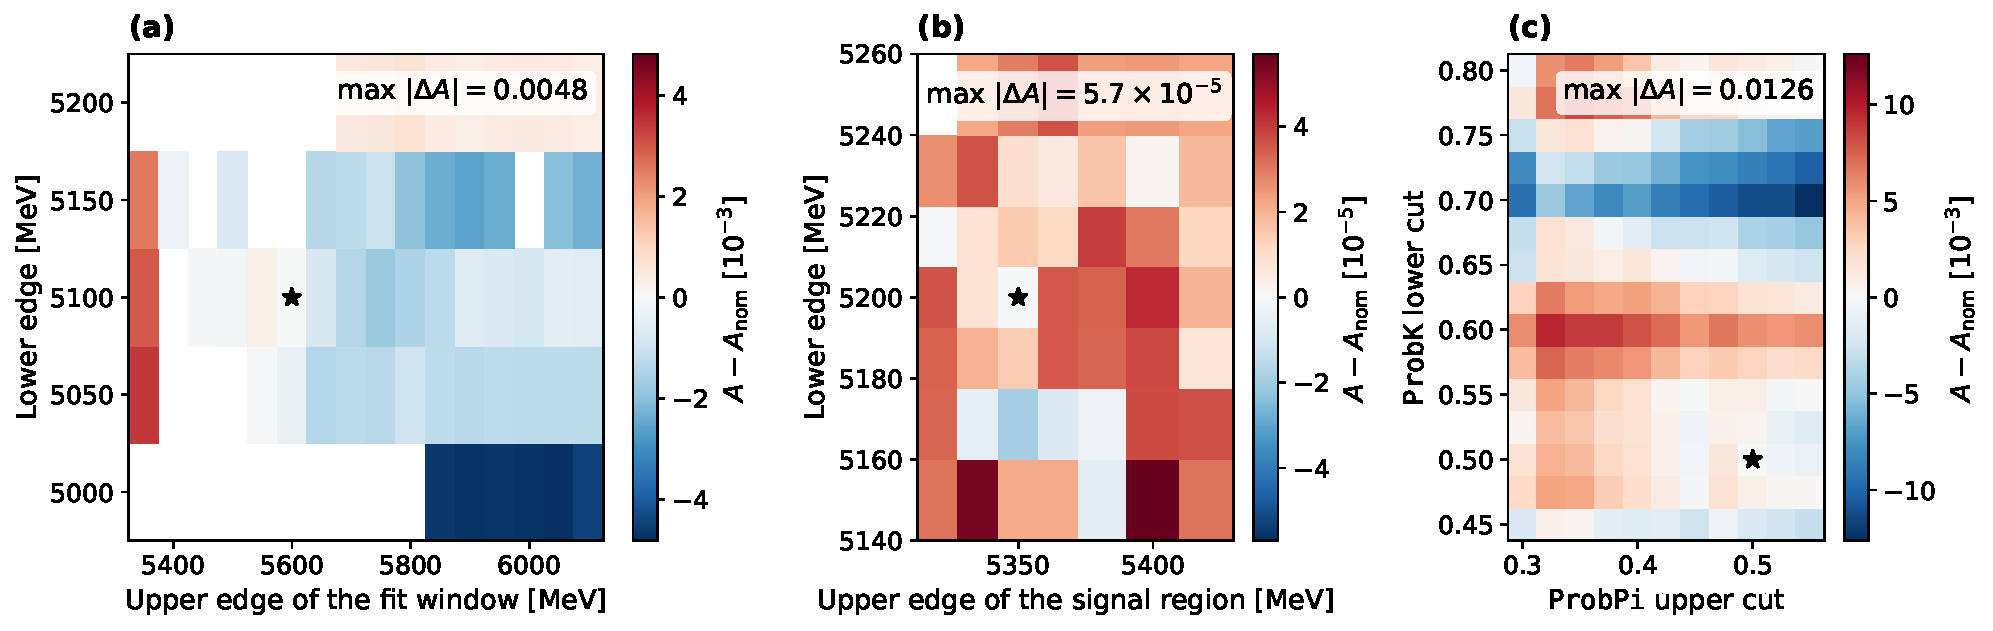
\includegraphics[width=0.95\textwidth]{figures/freq_stability.pdf}
\caption{Stability of the fitted $\Araw$ over the three grids: (a) lower and upper edge of the fit window (only fits with a valid minimum and an accurate covariance are shown); (b) lower and upper edge of the signal region; (c) lower cut on \texttt{ProbK} and upper cut on \texttt{ProbPi}. The colour is the shift with respect to the nominal fit (star), in units of $10^{-3}$ for (a) and (c) and $10^{-5}$ for (b); the statistical uncertainty of the nominal fit is $8.5\times10^{-3}$.}
\label{fig:freq_stability}
\end{figure*}

\subsection{All Fits of the Nominal Model and of Its Variants}
\label{sec:syst_tables}
\emph{In short: the Bayesian and Frequentist results of every variant and cross-check side by side.}

\subsection{Shifts of All Variants}
\label{app:syst_variants}
\emph{In short: the shifts of the Bayesian and Frequentist fits coincide variant by variant; the preselection group dominates, and the single exponential, rejected by the data, is drawn open.}
The $13$ variants of the systematic study (Sec.~\ref{sec:syst}) are shown in Fig.~\ref{fig:syst_variants}. For the variants that change the sample the bar is the expected statistical spread $\sigma_B$ of the shift (Sec.~\ref{sec:checks_barlow}); the others have no bar because the sample is the same. The Bayesian (purple) and Frequentist (green) shifts agree variant by variant, the preselection group is the largest, and the single exponential, which the data reject, is drawn open and excluded from the uncertainty.

\begin{figure}[t]
\centering
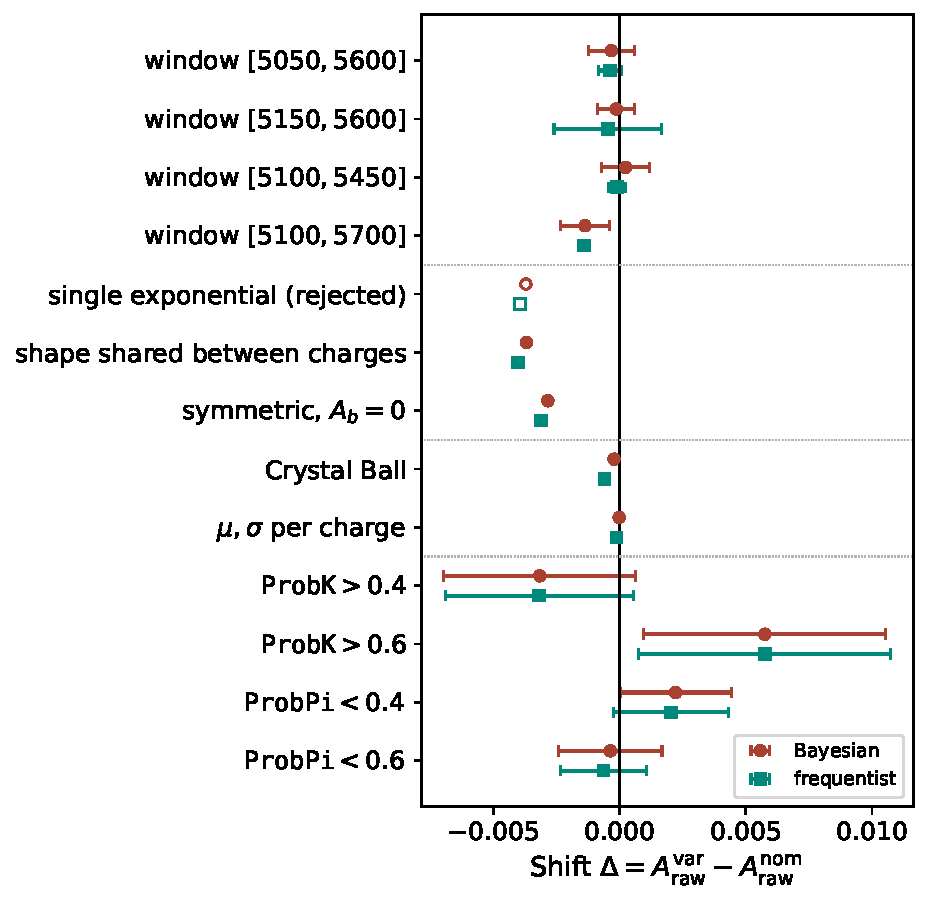
\includegraphics[width=\columnwidth]{figures/syst_variants.pdf}
\caption{Shift $\Delta=A_{\mathrm{raw}}^{\mathrm{var}}-A_{\mathrm{raw}}^{\mathrm{nom}}$ of every variant of the systematic study, Bayesian and Frequentist fits; bars: expected spread $\sigma_B$ of a nested subsample (variants that change the sample only). Open symbols: variant rejected by the data. The dotted lines separate the groups (window, background, signal, preselection).}
\label{fig:syst_variants}
\end{figure}

\subsection{Scan of the Particle-Identification Cuts}
\label{sec:syst_pid_scan}
\emph{In short: on the tight side the shift scatters around zero within $1.3\,\sigma_B$ and the pion requirement is flat; loosening $\texttt{ProbK}$ moves $\Araw$ monotonically, which supports the nominal requirement.}
A scan in steps of $0.05$ of each cut ($\texttt{ProbK}>0.30$--$0.85$, $\texttt{ProbPi}<0.15$--$0.70$) shows that on the tight side the shifts scatter around zero without a trend, all within $1.3\,\sigma_B$, and the pion requirement is flat: the $\texttt{ProbK}>0.6$ value is a statistical fluctuation and the preselection uncertainty is conservative. Loosening the kaon requirement moves $\Araw$ monotonically ($-0.0019$ to $-0.0111$ for $\texttt{ProbK}>0.45$--$0.30$, the last at $2.5\,\sigma_B$), as expected if misidentified $B\to K\pi\pi$ and $B\to\pi KK$ decays, not in the mass model, enter the sample; this supports the nominal requirement.
The scan is shown in Fig.~\ref{fig:syst_pid_scan}.

\begin{figure*}[!t]
\centering
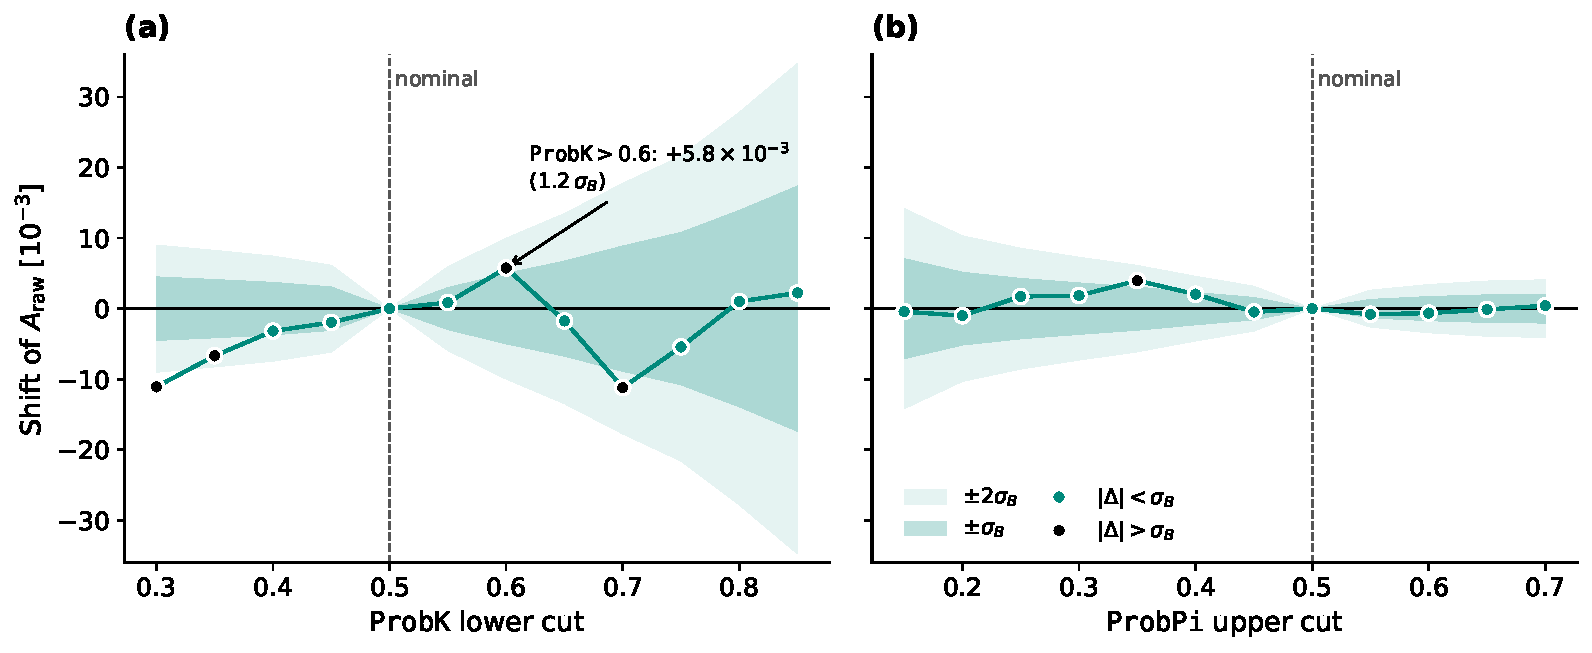
\includegraphics[width=0.85\textwidth]{figures/short_pid_scan.pdf}
\caption{Shift of $\Araw$ (Frequentist fit) as a function of (a) the $\mathtt{ProbK}$ lower cut and (b) the $\mathtt{ProbPi}$ upper cut, in steps of $0.05$, with the expected statistical spread of the nested sample ($\pm\sigma_B$ dark, $\pm2\sigma_B$ light); points beyond $\sigma_B$ are in red and the nominal cut is the dashed line. On the tight side of $\mathtt{ProbK}$ the points scatter around zero without trend and the pion requirement is flat; loosening $\mathtt{ProbK}$ moves $\Araw$ monotonically. The variant used in the systematic study, $\mathtt{ProbK}>0.6$, is a $1.2\,\sigma_B$ fluctuation.}
\label{fig:syst_pid_scan}
\end{figure*}

\subsection{Sensitivity of $\sigma_B$ to Differences between the Methods}
\emph{In short: $\sigma_B$ is the difference of two nearly equal uncertainties and is sensitive to small differences between the methods; a variant at the threshold can be classified differently without changing the result.}
Each method computes $\sigma_B$ from its own uncertainties (posterior standard deviation, Hesse error). Since $\sigma_B$ is the difference of two nearly equal uncertainties, it is sensitive to small differences between them, including the Monte Carlo noise of the posterior standard deviation (1--3\%), and a variant close to the threshold can be classified differently by the two methods: $\texttt{ProbPi}<0.4$ counts for the Bayesian fit ($|\Delta|=0.00223$, $\sigma_B=0.00220$) and not for the Frequentist one ($0.00204$ vs $0.00229$). This does not affect the result, since the uncertainty of each group is set by its largest shift, the same in both methods.
\subsection{Validation of the Rule for Nested Samples}
\label{sec:checks_barlow}
\emph{In short: the spread of the shift of $\hat A$ between a sample and its tighter-identification subsample is the one given by the quadrature difference of the uncertainties.}
The systematic study counts a variant that changes the sample only if its shift exceeds $\sigma_B=\sqrt{|\sigma_{\mathrm{var}}^2-\sigma_{\mathrm{nom}}^2|}$ (Sec.~\ref{sec:syst}). To verify the rule, $300$ bootstrap replicas of the nominal sample were fitted before and after the tighter selections $\texttt{ProbK}>0.6$ and $\texttt{ProbPi}<0.4$ (Fig.~\ref{fig:checks_barlow}): the standard deviation of the shift is $0.0051$ and $0.0025$, against median $\sigma_B$ of $0.0050$ and $0.0023$ (ratios $1.02$ and $1.09$), and the shifts follow a Gaussian of width $\sigma_B$. The mean shift of the replicas ($0.0060$ and $0.0020$) is that of the data, which is preserved by the resampling: it is a property of the sample and not a fluctuation of the rule.

\begin{figure*}[t]
\centering
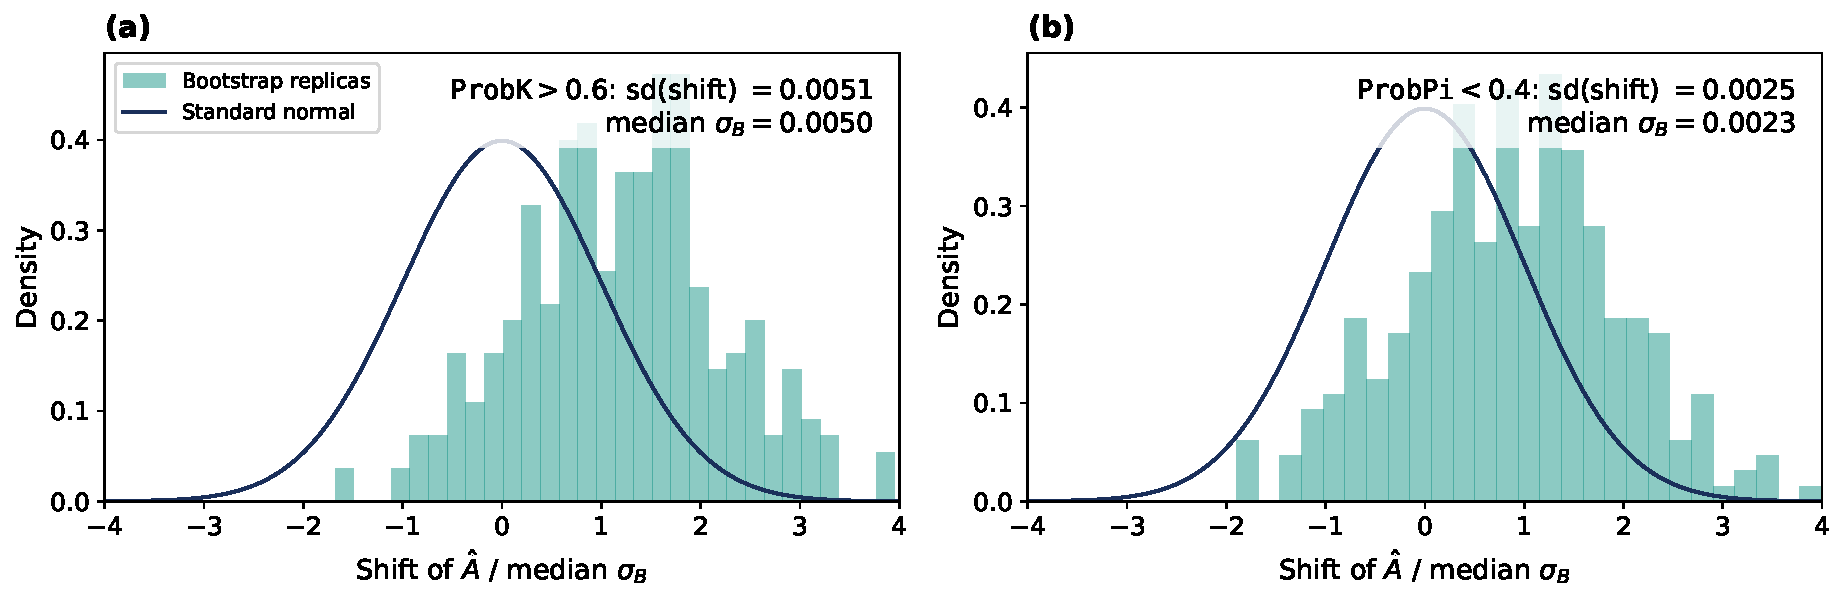
\includegraphics[width=0.95\textwidth]{figures/validation_barlow.pdf}
\caption{Shift of $\hat A$ between the nominal sample and a tighter selection, divided by the median $\sigma_B$, in $300$ bootstrap replicas of the data: (a) $\texttt{ProbK}>0.6$, (b) $\texttt{ProbPi}<0.4$, and standard normal distribution.}
\label{fig:checks_barlow}
\end{figure*}

